\subsection{Introduction}

The compact genome of \cer{} is covered by several machineries that need to be temporally and spatially coordinated to limit interferences that might affect robust reading and perpetuation of the genetic information. Transcription itself best exemplifies the complexity of the genomic landscape. Transcription initiation occurs frequently in regions and direction that largely overrun the annotations of genes with an assigned function \cite{david:2006:highresolution, xu:2009:bidirectional}. This is believed to be due to a leaky control on initiation and to the general of bi-directionality of promoters, which is also generally conserved in evolution. Transcription units largely overlap in both sense and antisense direction, and although RNA polymerases II (RNAPII) only seldom collide \cite{zenklusen:2008:singlerna}, the chromatin marks associated with ongoing transcription persist, and are susceptible to considerably impact concurrent transcription events. Overlapping transcription has also a large potential for regulation of gene expression, and is sometimes controlled and  tamed to the need of the cell \cite{martens:2004:intergenic}. 

The pervasive nature of transcription brings about two main potentially perturbing elements: the first is the presence of transcribing RNA polymerases which might directly affect other DNA-related events; the second is the production of many non-coding RNA molecules that might titer RNA-binding factors and indirectly affect gene expression. Cells possess tools to control both, by terminating “spurious” transcription events and degrade a large fraction of the RNA produced. In this perspective, transcription termination and RNA degradation, besides being devoted to the production of functional RNAs, additionally qualify as quality control mechanisms \cite[for review see][]{tudek:2015:noncoding}. 

In yeast, two main pathways of termination exist. The first is operated by a complex called the Cleavage and Polyadenylation Factor-Cleavage Factor (CPF-CF) and is used to arrest transcription of mRNA coding genes. The CPF-CF complex recognizes signals on the nascent RNA and cleaves it, producing a 5’ fragment that is polyadenylated by the Pap1 poly(A) polymerase and exported to the cytoplasms.  The 3’-fragment still associated to the transcribing polymerase is recognized and degraded by a \FtoT{} exonuclease,  Rat1, which contributes to dismantling the elongation complex by a much discussed but still unclear mechanism \cite{kim:2004:yeast}. The CPF-CF is also believed to be directly involved in termination by allosterically modifying the properties of the transcription elongation complex \cite{zhang:2005:ctddependent}. 
The second canonical pathway is dependent on the NNS (Nrd1-Nab3-Sen1) complex and was traditionally associated to the production of sn- and snoRNAs \cite{kim:2006:distinct}. Nrd1 and Nab3 bind the RNA at short motifs containing a well-conserved 4-5 nucleotides core \cite{carroll:2004:identification} and are thought to recruit Sen1 that translocates on the nascent RNA to release the polymerase by a mechanism that remains unclear \cite{porrua:2013:bacteriallike}. Peculiar to this pathway is the treatment of the RNA released, that is polyadenylated by a different poly(A) polymerase, Trf4, functioning within the TRAMP4 (Trf4-Air2-Mtrf4-Polyadenylation) complex, and trimmed to its mature size in the nucleus by the exosome, a large multisubunit complex that is endowed with 3’ to 5’ exonuclease activities \cite{vasiljeva:2006:nrd1}. 

A large share of the transcripts produced by pervasive transcription do not code for proteins and to what extent these RNAs have specific functions remains matter of debate. They are sorted in classes, generally defined by the pathways associated to their metabolism. CUTs (Cryptic Unstable transcripts) have been first described based on their extreme instability \cite{wyers:2005:cryptic}. These RNAs derive from transcription events terminated by the NNS pathway and are degraded to completion by the TRAMP-exosome pathway. When NNS termination is defective, elongated forms of CUTs are produced that are presumably terminated downstream by the CPF-CF pathway because they are insensitive to nuclear, exosomal degradation. These elongated forms of CUTs have been more recently named NUTs (Nrd1 Unterminated Transcripts) \cite{schulz:2013:transcriptome}.  Some of the non-coding RNAs produced by pervasive transcription are sufficiently stable to be detected in wild type cells (SUTs, stable unannotated transcripts \cite{david:2006:highresolution}) or are degraded in the cytoplasm by the nonsense-mediated decay (NMD) and Xrn1 pathways (XUTs, Xrn1-sensitive Unstable Transcripts \cite{vandijk:2011:xuts}). Finally, some are only detected in particular physiological conditions (MUTs,  meiotic unannotated transcripts \cite{lardenois:2011:execution}). 

We have recently described an additional pathway of transcription termination that depends on the DNA-binding protein Reb1 and that was dubbed road-block (RB) termination \cite{colin:2014:roadblock}. The elongating polymerase was shown to pause upstream of DNA-bound Reb1, which provokes its release by a mechanism that involves its ubiquitylation and presumably degradation. The isolated binding site of Reb1 was shown to be sufficient for eliciting termination when inserted in regions of active elongation, indicating that additional sequence elements are not required for efficient RB termination.  Because, akin to CUTs, the RNAs released are polyadenylated by TRAMP and degraded by the nuclear exosome, these transcripts where dubbed RUTs (Reb1-dependent Unstable Transcripts).  

In this report we demonstrate that several DNA-binding factors or complexes are able to terminate transcription by a RB mechanism. We generated high-resolution data on the distribution of RNAPII upon depletion of RB factors to address the significance and extension of RB termination at the genomewide scale.  We demonstrate that prominent peaks of roadblocked polymerases accumulate in intergenic regions immediately downstream of canonical terminators, indicating the significant occurrence of transcriptional readthrough in wild type cells. Akin to the leaky control on transcription initiation, the constitutive failure to terminate efficiently generates an additional level of pervasive transcription that has the potential to strongly affect the function of downstream regulatory regions or other DNA associated events. 
We show that RB and canonical termination pathways are not dependent on each other. High resolution analyses of RNAPII occupancy upon affecting either RB or CPF-CF and NNS termination indicates that RB is unlikely to partake in canonical termination and, conversely, that NNS and CPF-CF pathways are unlikely to be involved in RB termination. Rather, RB termination plays an important quality control role in limiting pervasive transcription events due to termination failure.  
The faculty of DNA associated factors to alter the processivity of elongation complexes, and the widespread occurrence of these factors defines a large potential in shaping and regulating the transcriptome. We propose that road-block termination constitutes an additional, general level of control on transcription that operates at the post-initiation level by altering the efficiency and extent of RNAPII elongation. 

\subsection{Results}

\singlespacing
\subsection*{\textit{In Vivo} Selection Reveals Rap1-Dependent Transcription Termination}
\doublespacing

We have previously described a procedure to select transcription terminators from pools of naïve sequences \cite{porrua:2012:in}. Briefly, test sequences are inserted within a transcription unit driven by the tetracycline-repressible (TetP) promoter, roughly 200nt downstream of the transcription start site. A second promoter from the GAL1 gene is inserted downstream and drives expression of a selectable marker, CUP1, the expression of which is required for yeast growth in copper-containing medium. In the absence of a terminator in the test sequences, transcription driven from TetP silences the GAL1 promoter by transcription interference and prevents CUP1 expression, which leads to copper-sensitivity. When the test sequence induces termination, the CUP1 gene is expressed and yeasts grow on copper-containing plates (Fig. \ref{fig:one}A). 
Using this system we selected terminators from a pool of sequences containing a stretch of 120 random nucleotides. We selected many sequences inducing termination via the NNS pathway and via the Reb1-dependent road-block pathway. We also selected sequences that do not belong to either class, some of which contain a motif resembling a Rap1 binding site (Figure \ref{fig:one}B). Rap1 recognizes its site via a Myb-like DNA-binding domain and is involved in many DNA-associated processes, including telomere maintenance and gene expression. Rap1 is also strongly associated to the positioning and formation of nucleosome free regions (NFR). 

\begin{figure}[hp!]

\centering
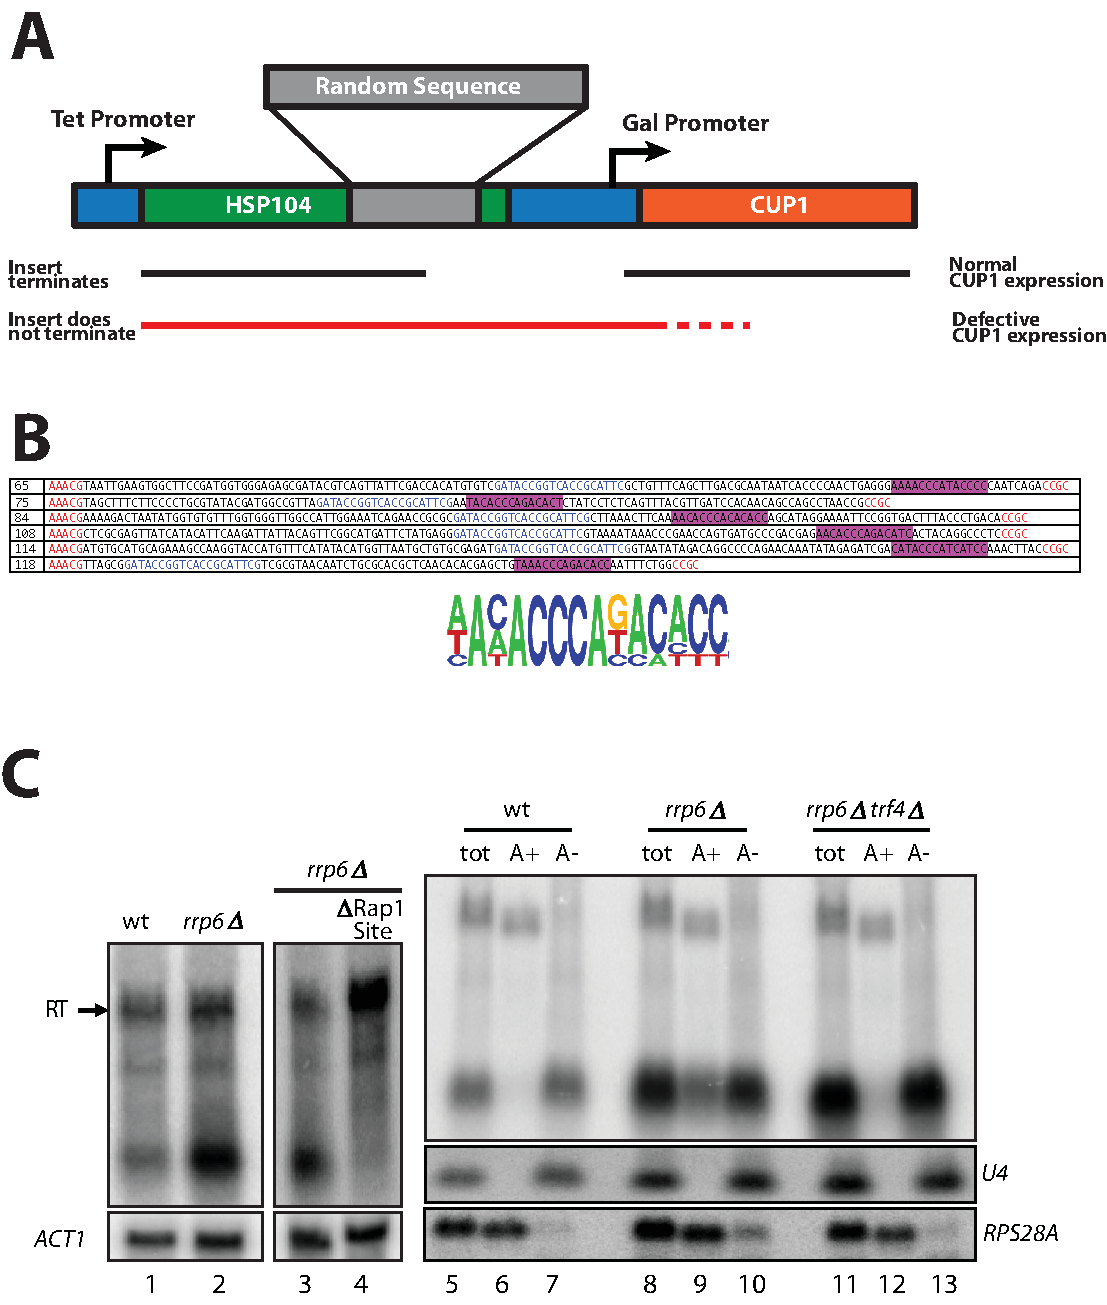
\includegraphics[width=\textwidth]{figures/results/rap/one.pdf}
\caption[Rap1-dependent transcripts are isolated from \invivo{} selection]{\textbf{A: }Schematic representation of the reporter system used to select Rap1-terminated transcripts. \textbf{B: }Sample of selected sequences containing Rap1 sites, the identified consensus is represented. \textbf{C: }Northern blot analysis of several species derived from the reporter system.}
\label{fig:one}

\end{figure}


It has previously been shown that the presence of a Rap1 binding site can induce RNAPII stalling in a model Ty1 retrotransposon construct \cite{yarrington:2012:novel}. In this study, the occurrence of Rap1-dependent transcription termination was ruled out based on the analysis of the transcripts produced in the presence of the Rap1 site. These RNAs were non-adenylated and insensitive to nuclear degradation, and therefore assumed to be nascent RNAs associated to the stalled polymerase. Moreover, it was not demonstrated that stalling is dependent on the integrity of Rap1 or its binding to the DNA.
The stalling model would hardly be compatible with our results, because only loss of polymerases – and therefore termination – is expected to prevent transcription interference. We therefore assessed whether the presence of the selected site would induce Rap1-dependent transcription termination. We first demonstrated that the Rap1 binding site is necessary and sufficient to prevent transcription interference at the GAL1 promoter. Indeed, mutation of the site in the context of a selected clone prevented yeast growth on copper, while insertion of the site in a fragment of the coding region of the HSP104 gene was sufficient to induce copper resistance (data not shown).  


These results were confirmed by direct analysis of the RNA produced. To assess whether the transcripts released undergo nuclear degradation, we analyzed the RNAs in both a wt and degradation-defective rrp6∆ and trf4∆ strains. As shown in figure \ref{fig:one}C, a short RNA is produced when a selected terminator is present in the reporter construct. For all of the terminators analyzed, the size of this RNA is 13-17 nt shorter than the distance between the transcription start site and the Rap1 site (data not shown), suggesting that stalling or release of the polymerase occurs upstream of the site, which is consistent with a road-block mechanism. 

The transcripts produced are strongly sensitive to degradation, as indicated by their marked steady state increase when the analysis is performed in a ∆rrp6 exosome mutant (Figure \ref{fig:one}C, lanes 1-2). This indicates that these transcripts cannot solely correspond to polymerase-associated nascent RNAs but rather that they are released upon transcription termination. The short transcript disappears to the profit of a longer, read-through product when the Rap1 site is deleted (compare lanes 3 and 4) The bulk of the transcripts released and degraded appears to be non-adenylated (Figure \ref{fig:one}C, compare lanes 7, 10 and 13), although a fraction is polyadenylated by Trf4 (compare lanes 9 and 12). The transcripts that are detected in a wild type strain are non-adenylated (lanes 5-7) and might correspond to nascent RNAs that are protected from degradation because of their association with the polymerase.

The dependency on the Rap1 site strongly suggests, but does not prove that Rap1 is involved in termination. Indeed, termination might occur via other pathways, e.g. as a result of the recognition of partially or fully overlapping termination signals at the Rap1 site.  To prove the Rap1 dependency, we transiently depleted this essential factor with the anchor away strategy and analyzed the transcripts produced. As shown in figure \ref{fig:two}A, the levels of the short RNA derived from the reporter construct are markedly decreased in the absence of Rap1, to the profit of a longer species earmarking termination at a downstream site. From this result we conclude that Rap1 is necessary to induce termination at the selected sites. 

Finally, we have previously shown that release of the road-blocked polymerase from the DNA template occurs following its ubiquitylation that depends on the Rsp5 ubiquitin ligase. When the elongation complex is dismantled, the RNA released is polyadenylated and degraded rapidly; conversely, the persistence of roadblocked RNAPII on the DNA template following mutation of Rsp5 leads to an increase of the nascent, non-adenylated transcript that can be detected in a wild type strain \cite{colin:2014:roadblock}. Northern blot analysis confirmed the expected increase in the levels of nascent RNAs when the Rap1-roadblocked polymerase is less efficiently removed in a thermosensitive rsp5-1 mutant strain (Fig. \ref{fig:two}B). 

This finding is also substantiated by the observation that recombinant Rap1 binds very efficiently the double stranded DNA but not the RNA or single stranded DNA version of its site (supplementary figure \ref{fig:S2}). 

Together, these results demonstrate that transcription termination occurs by a road-block mechanism at sites bound by Rap1. 

\begin{figure}[hp!]

\centering
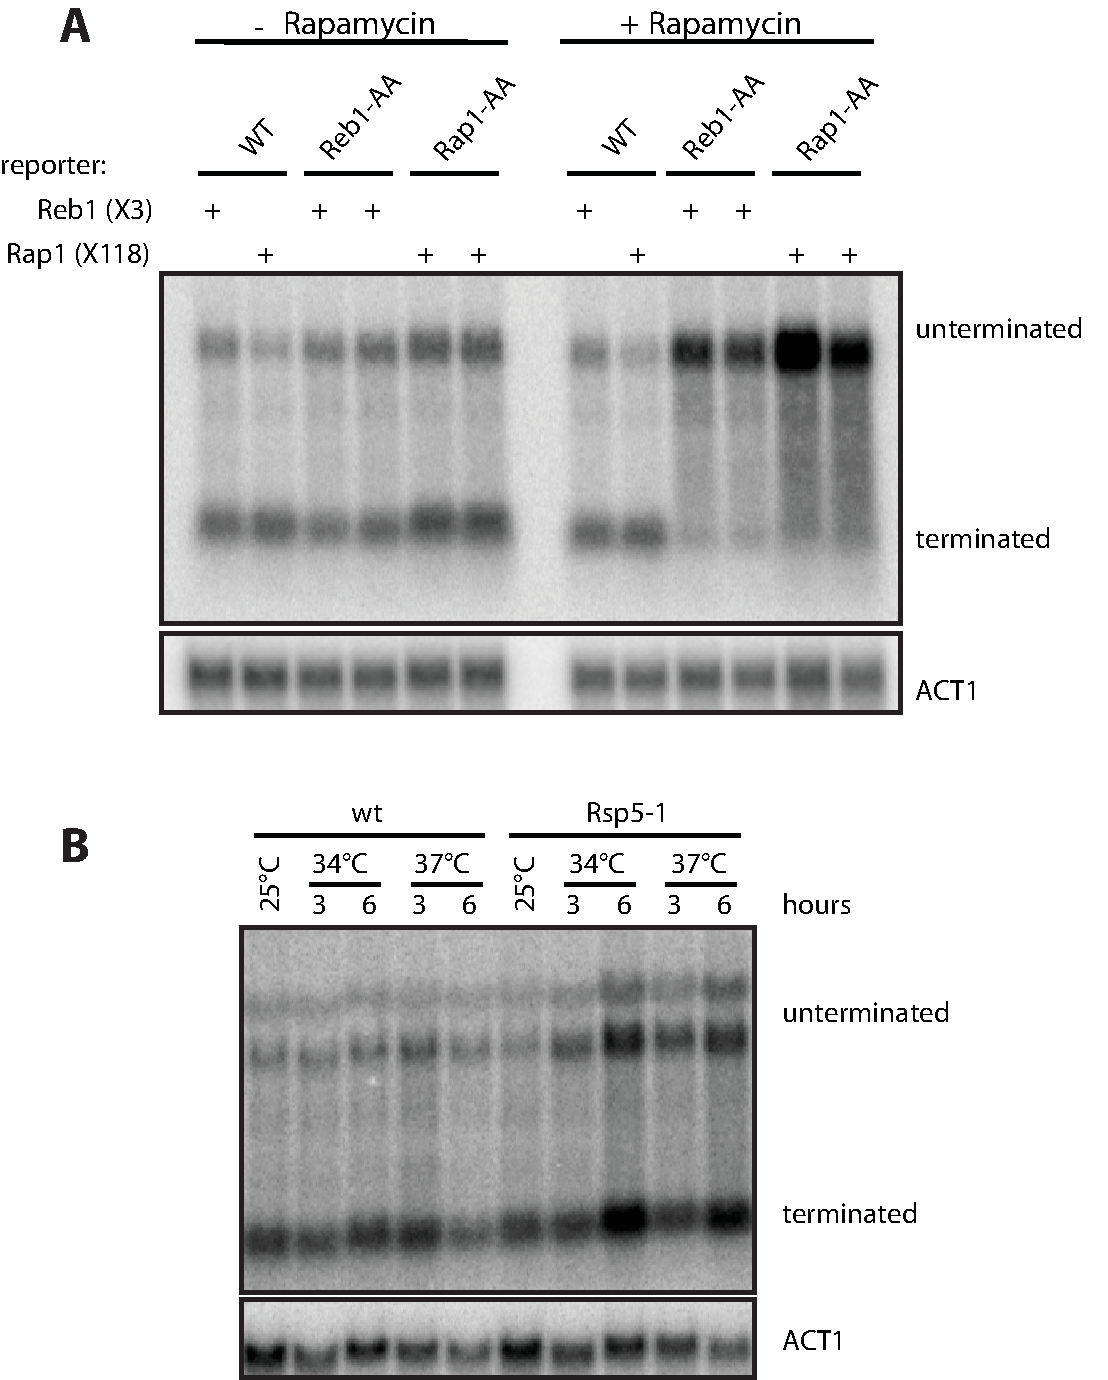
\includegraphics[width=\textwidth]{figures/results/rap/two.pdf}
\caption[dfgdf]{\textbf{A: }Northern blot analysis in presence or absence of Reb1 and Rap1 of specific sequences containing Reb1 or Rap1 terminators. \textbf{B: }Norther blot analysis of Rap1-terminated transcripts in a strain containing thermosensitive ubiquitin ligase Rsp5. }
\label{fig:two}

\end{figure}

\singlespacing
\subsection*{Rap1-Dependent Transcription Termination in the \cer{} Genome}
\doublespacing

These results constitute the proof-of-principle that transcription termination can occur in a Rap1-dependent manner, but do not prove that it occurs significantly in the \cer{} genome. A hallmark of road-block termination is the accumulation of RNAPII immediately upstream of the site of road-block, due to polymerase pausing. 

We therefore assessed whether RNAPII pausing can be observed in the \cer{} genome at Rap1 sites and whether pausing would be dependent on Rap1. To this end, we analyzed the RNAPII distribution in a wild type and a Rap1 anchor away (Rap1-AA) strain by a modified crosslinking and cDNA analysis (CRAC) method \cite{bohnsack:2012:identification, granneman:2009:identification}. By this approach, the position of the polymerase is directly inferred by sequencing the nascent transcript associated to the largest subunit of the enzyme after \invivo{} UV crosslinking \cite{milligan:2016:strandspecific}. Consistent with the notion that the signals obtained genuinely represent nascent and not mature transcripts, intronic regions where largely covered in the RNAPII CRAC dataset but not in the sequencing of mature, total RNAs (supplementary figure \ref{fig:S3}).

\begin{figure}[hp!]

\centering
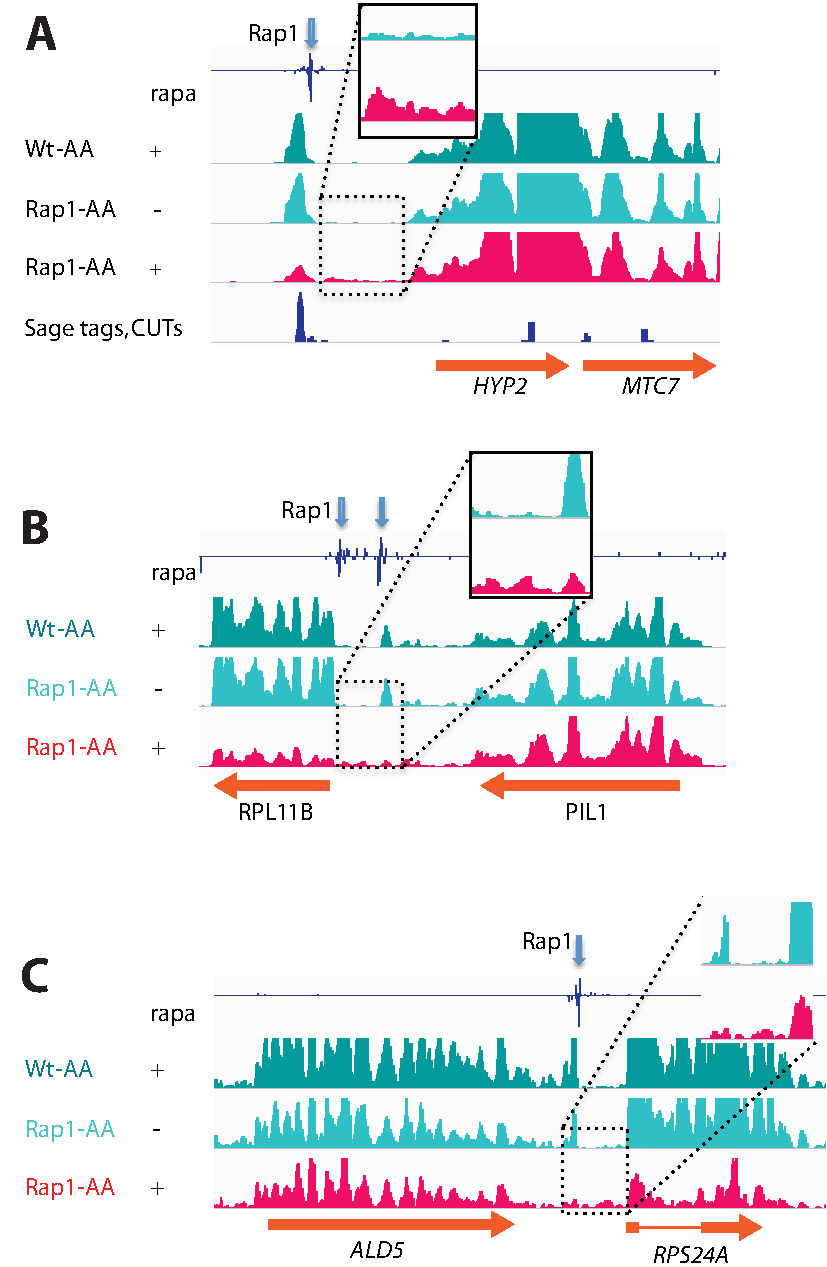
\includegraphics[width=\textwidth]{figures/results/rap/three.pdf}
\caption[Examples of Rap1-dependent termination detected \invivo{}]{Examples of Rap1-dependent termination detected \invivo{} through the CRAC technique. RNAPII occupancy signal accumulates upstream of Rap1 binding sites in wild type. This occupancy peak is reduced upon the addition of rapamicing to the Rap1-AA strain.}
\label{fig:three}

\end{figure}

In the Rap1-AA strain, Rap1 is rapidly and efficiently depleted from the nucleus upon addition of rapamycin \cite{haruki:2008:anchoraway}.  Notable examples of sites of Rap1-dependent road-block sites are shown in figure \ref{fig:three}. Two Rap1 binding site are present upstream of the HYP2 gene and constitute a prominent site of Rap1 localization as detected by several techniques \cite{rhee:2011:comprehensive, kubik:2015:nucleosome}. CRAC analysis reveals a prominent accumulation of the RNAPII signal immediately upstream of the Rap1 sites, indicating pausing. The occurrence of termination is demonstrated by the existence of a non-annotated unstable transcript ending in correspondence of the RNAPII peak, revealed by microarray analysis \cite{neil:2009:widespread} and by a cluster of 3’-end SAGE. RNAPII pausing and termination were Rap1-dependent, because depletion of Rap1 led to a strong reduction in the RNAPII peak and to the appearance of a readthrough signal downstream of the site (Fig. 3A, inset). Finally, insertion of the two Rap1 sites in the heterologous context of our reporter system induced Rap1-dependent termination and led to the production of an unstable RNA (supplementary figure \ref{fig:S4}).

Two other examples are shown in figure \ref{fig:three}B-C. In these cases, the Rap1 occupancy site is located between two tandem genes and the accumulation of RNAPII is most likely due to transcription events reading through the upstream terminator (see below). In both cases, depletion of Rap1 leads to abrogation of the peak and increased RNAPII signals downstream of the site (Fig. \ref{fig:three}B-C, insets). 

To extend these results to a genomewide perspective we profiled the average distribution of the RNAPII CRAC signal around aligned sites of Rap1 occupancy found in promoter regions.

\begin{figure}[h]

\centering
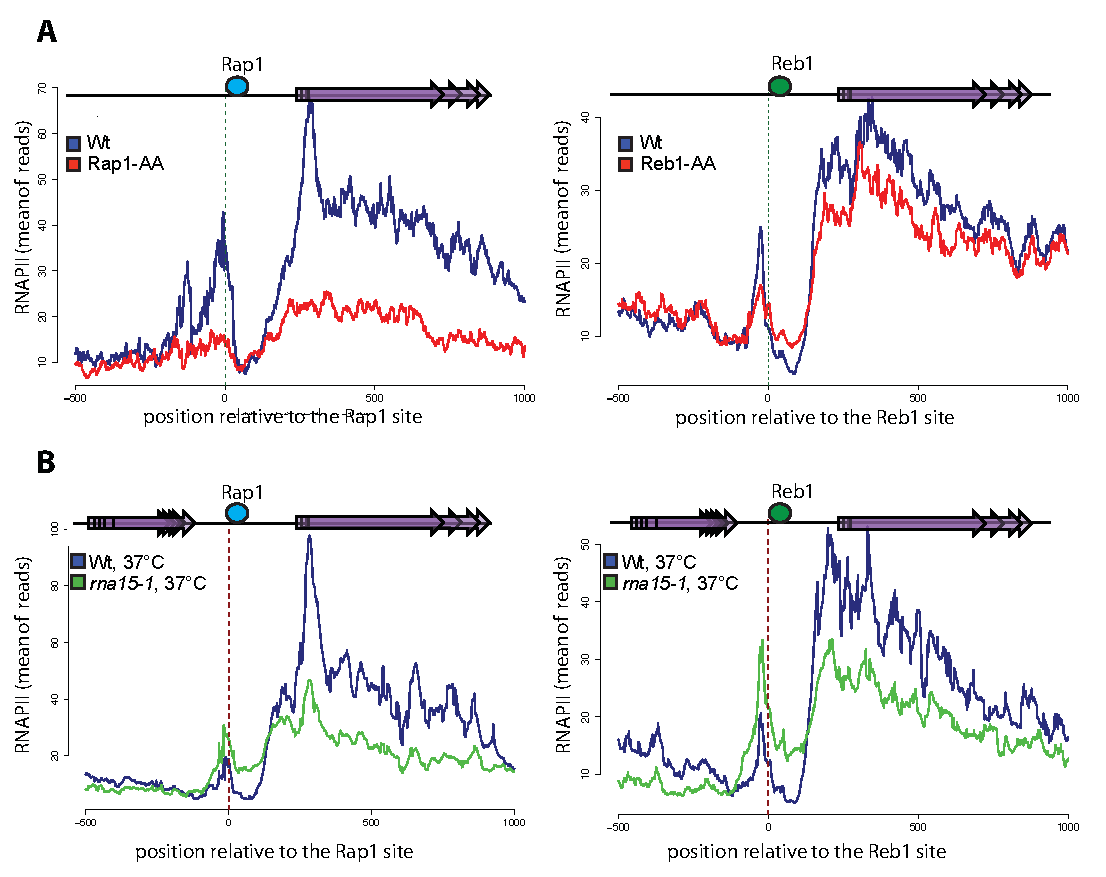
\includegraphics[width=\textwidth]{figures/results/rap/four.pdf}
\caption[Metagene analysis around sites of Rap1 and Reb1.]{Metagene analysis around sites of Rap1 and Reb1. \textbf{A: }Global view of polymerase occupancy around sites of Rap1 residing in promoter regions. in Rap1-AA, the pause associated with the site decreases significantly. \textbf{B: }Global view of polymerase occupancy around sites of  Rap1 that follow  a CPF-terminated transcript. Upon inactivation of rna15, the readthrough from the upstream transcripts accumulates in front of the road-block site. \textbf{C and D: }The same analyses were performed with Reb1 sites.}
\label{fig:four}

\end{figure}

Rap1 is required for the strong expression of ribosomal protein (RP) genes, and is often positioned in nucleosome free regions (NFRs) upstream of these genes. Consistently, a major peak of RNAPII occupancy is observed downstream of the aligned Rap1 binding sites, corresponding to the occurrence of transcription initiation within a relatively short window (Fig. \ref{fig:four}A and B). Importantly, however, a significant peak demonstrating RNAPII pausing is also observed upstream of Rap1 binding, which is associated to the occurrence of transcription termination in the same region (see below). Importantly, sequestering Rap1 out of the nucleus led to a significant decrease in the RNAPII pausing peak demonstrating that Rap1 dependent road-block occurs at many sites of Rap1 binding in the genome.

Similar RNAPII CRAC analyses were also performed upon Reb1 depletion (Fig. \ref{fig:four}C and D). Peaks of RNAPII pausing were readily observed at individual sites of Reb1 occupancy that disappeared upon Reb1 depletion (supplementary figure \ref{fig:S5} and data not show). Because Reb1 is also required for the expression of many genes, profiling RNAPII distribution around aligned sites of Reb1 occupancy revealed a similar transcription initiation peak as for Rap1.  Importantly, a prominent peak indicating RNAPII pausing was also observed upstream of Reb1 that strongly decreased upon sequestering Reb1 out of the nucleus. Overall, these results demonstrate the significant occurrence of Rap1- and Reb1-dependent, road-block transcription termination in \cer{}.





\singlespacing
\subsection*{Widespread Redundancy in Transcription Termination}
\doublespacing

In the compact \cer{} genome, efficient and timely release of the elongation complex is essential to prevent interference between contiguous transcription units. Whether CPF termination is inherently highly efficient or enforced by redundant mechanism remains unclear. Many sites of Reb1 and Rap1 occupancy are located in intergenic regions, downstream of genes terminated by the CPF pathway. If significant transcriptional read through occurs at these CPF terminators, polymerases are expected to be roadblocked at downstream sites of Reb1 and Rap1 occupancy, as also suggested in the cases of PIL1 and ALD5 (Fig.  \ref{fig:three}B-C). We therefore restricted our metasite analyses to Reb1 and Rap1 occupancy sites located within 300nt downstream of mRNA-coding genes. In these conditions, only polymerases escaping termination (if any) are expected to contribute to the metaprofile observed. As shown in figure \ref{fig:four}B and D, transcriptional road-block is clearly observed in the wild type strain at sites of Rap1 and Reb1 occupancy downstream of canonical CPF terminators. To prove that roadblocked polymerases indeed originate from readthrough at upstream terminators and not from spurious initiation between terminators and the road-block sites, we also performed a parallel RNAPII CRAC analysis using a thermosensitive rna15-1 allele, which impairs CPF termination.  A prominent increase in the road-block peak was clearly observed upon impairing CPF termination in the rna15-1 mutant, consistent with the notion that the flux that aliments roadblocked polymerases originates from upstream transcription units and increases when upstream termination is defective. As a control, we profiled RNAPII distribution at the same set of genes using published PAR-CLIP data obtained upon nuclear depletion of Nrd1 \cite{schaughency:2014:genomewide}, an essential actor of NNS termination that is not involved in termination of mRNA coding genes. In these conditions we did not observe an increase in the road-block peak (supplementary figure \ref{fig:S6} and data not shown) confirming that roadblocked polymerases originate from upstream, CPF-dependent genes. 
Although less prominent, road-block was also observed at sites of Abf1 occupancy downstream of CPF terminators, which increased, as for Rap1 and Reb1, when termination was impaired in an rna15-1 mutant (supplementary figure \ref{fig:S7}). 

Overall, these results demonstrate the widespread occurrence of significant levels of transcription readthrough at CPF terminators in strains that are proficient for transcription termination. This results in the constitutive accumulation of roadblocked polymerases at sites of Rap1 and Reb1 occupancy (and many additional sites in the genome, see below).


\singlespacing
\subsection*{Roadblock is Not Part of the CPF Termination Mechanisms}
\doublespacing


Although these results strongly suggest that road-block termination acts to neutralize transcriptional readthrough downstream of CPF-dependent terminators, it cannot be excluded that roadblocking the polymerase is an important requirement for efficient termination at the upstream canonical sites. For instance, it can be envisioned that pausing induced by the road-block favors chasing of the polymerase by Rat1. In this perspective, it is expected that reducing the road-block should affect the efficiency of termination at the upstream sites. To address this possibility, we investigated whether increased transcriptional readthrough could be observed at CPF terminators in the absence (or strong reduction) of the downstream road-block. We analyzed the level of polymerase in the region immediately downstream of CPF terminators in Reb1 or Rap1 anchor away strains upon nuclear depletion of either factor. Three examples of CPF-dependent genes with a downstream road-block are shown in supplementary figures \ref{fig:S8}. In all occurrences, transcription termination occurred efficiently at the CPF sites even in the absence of the road-block as witnessed by a very similar RNAPII signal at and downstream of the termination region. 

To generalize these observations, we first compared the RNAPII metaprofiles in regions of CPF termination upstream of a Rap1 binding sites in the presence and absence of the road-block factor. To this end we aligned for each gene the strongest site of poly(A) addition as defined by TIF-seq analyses \cite{pelechano:2013:extensive}, trusting that this will allow a sufficiently precise approximation of the average termination region. A decrease in the average RNAPII signal was observed in wild type cells in this region, confirming the progressive occurrence of termination. Depletion of Rap1 had no impact on the distribution of the RNAPII signal that declined in the termination region very similarly to the wild type indicating identical efficiencies of termination at the upstream CPF sites (Fig. \ref{fig:five}B). As a control, a termination defect could clearly be observed in rna15-1 cells at the non-permissive temperature (Fig. \ref{fig:five}A). Similar results were obtained for the set of CPF-dependent genes upstream of a Reb1-dipendent road-block (data not shown). 

\begin{figure}[h]

\centering
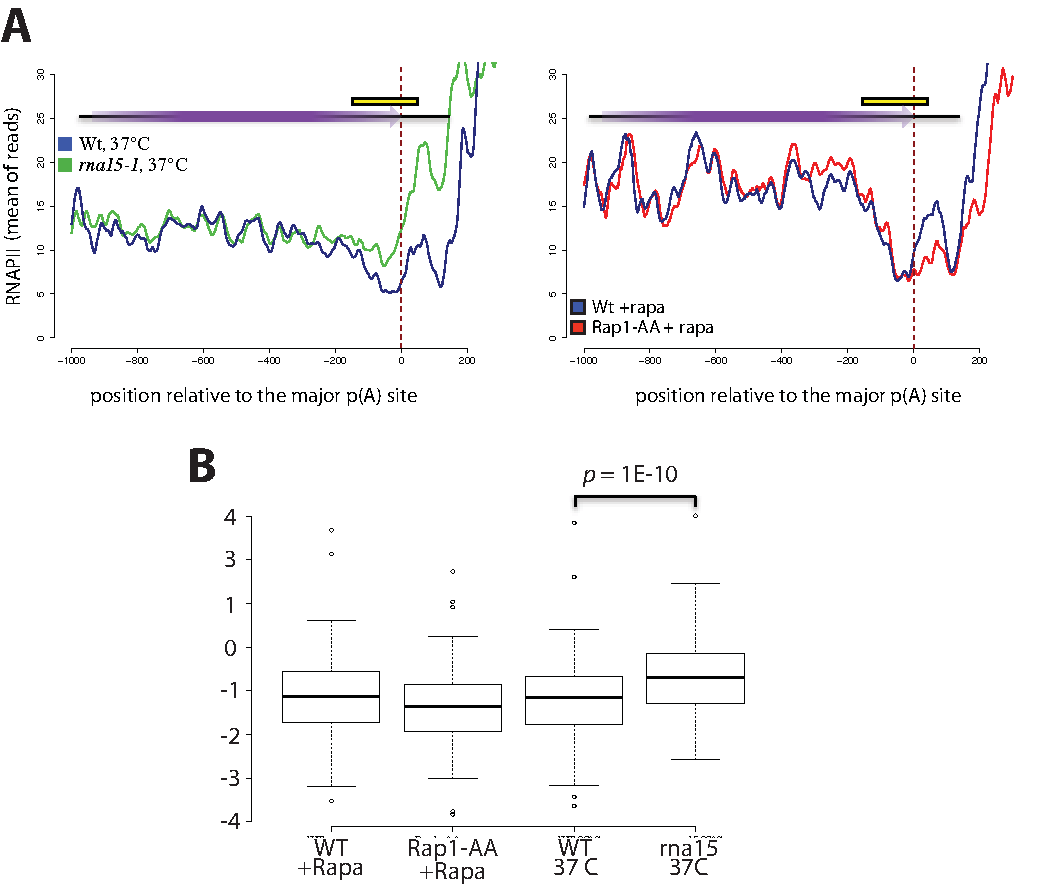
\includegraphics[width=\textwidth]{figures/results/rap/five.pdf}
\caption[Metagene analysis around poly(A) sites that are within 300bp upstream of Rap1 sites.]{Metagene analysis around poly(A) sites that are within 300bp upstream of Rap1 sites. \textbf{A: }Comparison of RNAPII average profile in wild type and rna15-1 at non-permissive temperature and \textbf{B: }the same analysis performed in wt or Rap1-AA strains. \textbf{C: }Comparison between ratios of RNAPII signal in the termination zone divided by RNAPII signal in the body of the gene. While a significant difference is detectable between rna15-1 and wt at non-permissive temperature, no such difference is detectable when Rap1-AA is compared with wt.}
\label{fig:five}

\end{figure}

To substantiate these results we calculated the fractional level of readthrough for each CPF-dependent gene upstream of a Rap1- dependent road-block by dividing the density of reads in the termination region by the density in the gene body. The distribution of the values obtained is strongly affected by the rna15-1 mutation, as expected for a bona fide termination defect ($p$=1E-8), but not by the absence of Rap1, demonstrating that the road-block does not significantly impact CPF termination (Fig. \ref{fig:five}C). 

\singlespacing
\subsection*{Roadblock and NNS-Dependent Termination}
\doublespacing

While this work was in progress another study suggested that road-block- and NNS-dependent termination are functionally linked, notably that: i) road-block is part of the mechanism of snoRNA termination and ii) that roadblocked polymerases are released by the NNS pathway. This study relied on the analysis of transcripts produced in different mutant conditions and on the published distribution of polymerases in wt and Nrd1 anchor away strains \cite{roy:2016:common}. We undertook to revisit this important question using our high-resolution RNAPII CRAC in cells defective for the CPF, NNS and road-block pathways. 

\begin{figure}[hp!]

\centering
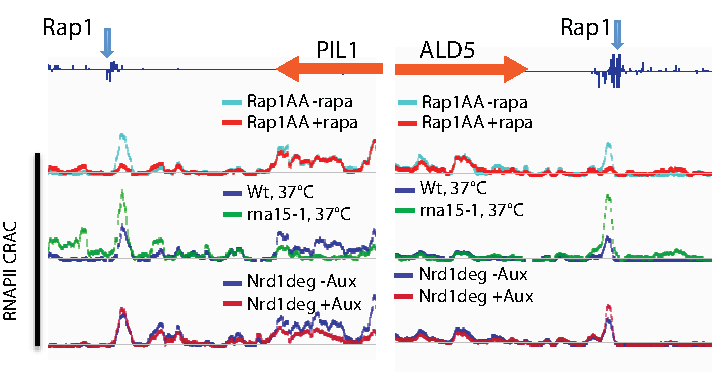
\includegraphics[width=\textwidth]{figures/results/rap/six.pdf}
\caption[Examples of CPF-terminated transcripts followed by sites of Rap1]{Examples of CPF-terminated transcripts followed by sites of road-block in the contex of Ra1-AA, rna15-1 and Nrd1-degron strains. the position of Rap1 sites and annotation of the transcripts is displayed at the top.}
\label{fig:six}

\end{figure}

Roadblock peaks have been shown to increase in strains defective for NNS termination, which was interpreted as evidence of defective clearing of roadblocked polymerases when NNS termination is impaired \cite{roy:2016:common}. An alternative interpretation, which we favor, is that when NNS termination is defective, polymerases that do not terminate at primary NNS termination sites accumulate downstream at road-block sites.  Consistent with this notion is the finding that the level of roadblocked polymerase is not sensitive to NNS termination at road-block sites preceded by CPF terminators (supplementary figure \ref{fig:S6}). Two such examples are shown in figure \ref{fig:six}. The RNAPII road-block peak increases considerably when CPF termination is impaired at the PIL1 and ALD5 loci but is unaffected by depletion of NRD1. Identical results were obtained at these loci when Sen1 was depleted (data not shown). Conversely, depletion of Nrd1 leads to an increase of the road-block peaks at Reb1 and Rap1 sites located downstream of NNS terminators (supplementary figure \ref{fig:S9}). Together, these results indicate that roadblocked polymerases are not generally released by the NNS pathway. 

\begin{figure}[h]

\centering
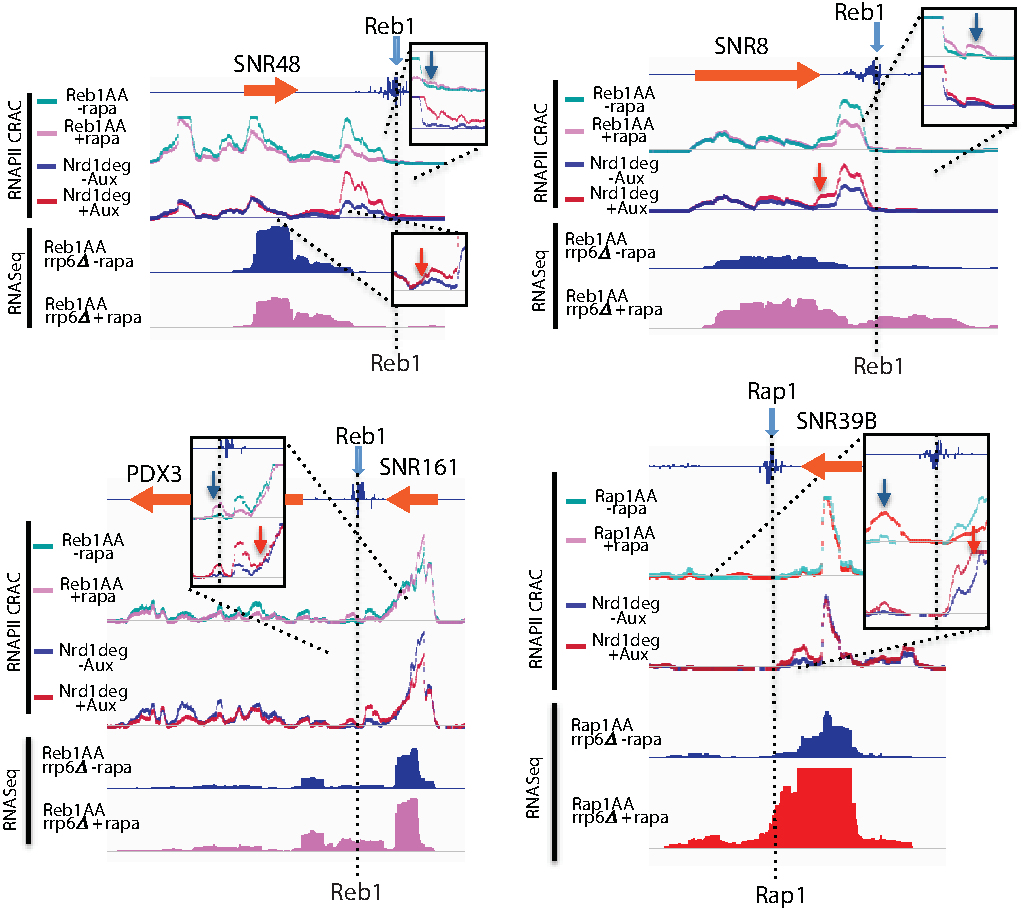
\includegraphics[width=\textwidth]{figures/results/rap/seven.pdf}
\caption[Analysis of 4 snoRNAs followed by road-block by CRAC and RNA-seq in several mutant strains.]{Analysis of 4 snoRNAs followed by road-block by CRAC and RNA-seq in several mutant strains. Position of the Reb1 or Rap1 site, and annotation of the transcripts is represented at the top of each image. Insets are elargements of the highlighted area.}
\label{fig:seven}

\end{figure}

In a small number of snoRNAs the road-block is located very near to the NNS terminator and it is possible that it contributes to the formation of a functional RNA. We analyzed the polymerase profile around four of these snoRNAs for which a Reb1- (SNR161, SNR8, SNR48) or Rap1-dependent (SNR39B) road-block peak of variable intensity was observed in the termination region. Depletion of Nrd1 led to a clear increase of the road-block peak, as expected. However, a clear increase in RNAPII occupancy was also observed between the NNS terminator and the region of the road-block (figure \ref{fig:seven}, red arrowheads), indicating the existence of a readthrough at the primary terminator that feeds the flow of polymerases accumulating later at the road-block. This was clearly visible at the SNR8 and SNR48 loci, where the road-block is slightly more distal (Fig. \ref{fig:seven}, panels A-B), but also observed at SNR161 and SNR39B where the signal due to the readthrough increase somewhat merged with the road-block peak (Fig. \ref{fig:seven} C-D).



Conversely, no evidence of readthrough could be observed at the primary termination site when the road-block factor (Rap1 or Reb1) was depleted, which only led to the expected decrease in the road-block peak.  A small but clearly visible readthrough extended downstream of the road-block (Fig. \ref{fig:seven}, blue arrowheads), most likely due to the release of polymerases accumulating at the failsafe site.   

We also analyzed the RNAs produced in the absence of the road-block (Fig. \ref{fig:seven}). We depleted Reb1 or Rap1 in an rrp6∆ strain, which allowed visualizing the primary product of transcription that is stabilized in this genetic context. Interestingly, in spite of the overall low level of polymerases going through the road-block site in the absence of Reb1 or Rap1, a significant increase in the amount of pre-snoRNA was generally observed (Fig. \ref{fig:seven}, see the RNAseq profiles at SNR8, SNR161 and SNR39B loci; data not shown), suggesting that transcription events terminating downstream of the road-block produce transcripts that are generally more stable than those produced by transcription terminating at the primary (NNS) or secondary (road-block) terminator. The levels of the mature snoRNAs were generally increased or unchanged in the absence of the road-block (data not shown), although the general stability of these forms prevents from drawing strong conclusions in these transient depletion experiments.  

These experiments strongly suggest that the absence of the road-block does not prevent the production of functional snoRNAs but allows the production of stable transcripts derived from a low level of readthrough transcription at the primary NNS terminator. Importantly they strongly support the notion that road-block termination functions as a fail-safe mechanism for both the CPF and the NNS pathways.


\singlespacing
\subsection*{Functional Importance of Fail-Safe Transcription Termination }
\doublespacing

\begin{figure}[hp!]

\centering
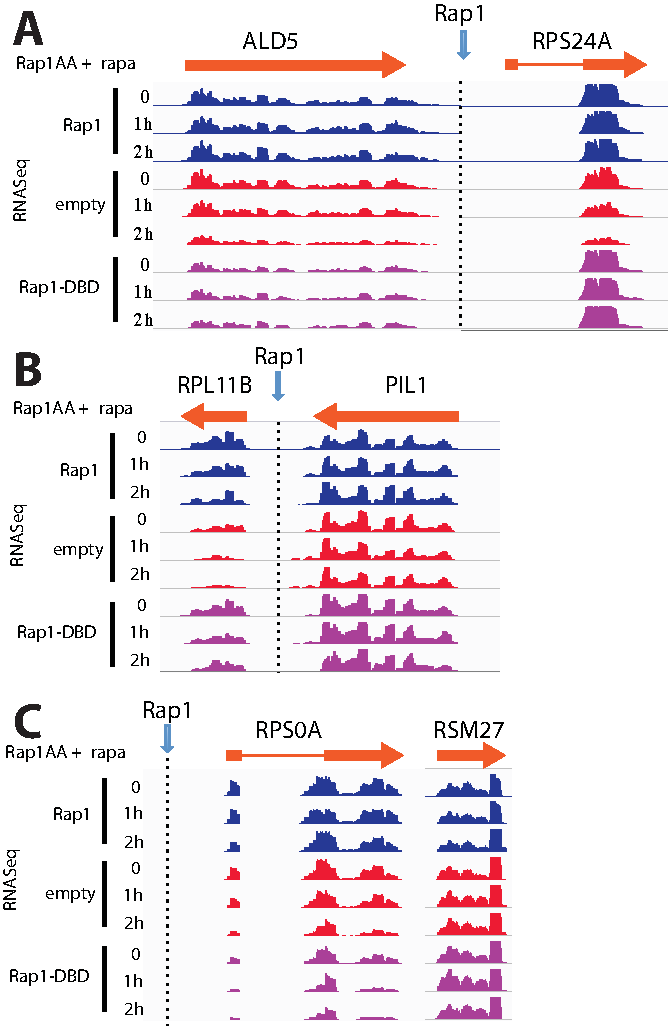
\includegraphics[width=0.85\textwidth]{figures/results/rap/eight.pdf}
\caption[RNA-seq analysis of genes followed by Rap1 sites.]{RNA-seq analysis of genes followed by Rap1 sites. \textbf{A: }Strains depleted for Rap1 were rescued with different plasmids, one expressing the full length Rap1, one expressing only the DNA-binding domain of Rap1, and an empty plasmid. The transcript downstream of the Rap1 site is downregulated in absence of the full length protein, but expression is rescued by the presence of the DNA binding Domain of Rap1. \textbf{B: }Rap1 site without an upstream feature. The same downregulation is detected in presence of both the empty plasmid and Rap1-DBD, thus proving that Rap1-DBD cannot activate transcription.}
\label{fig:eight}

\end{figure}

As shown in figure \ref{fig:eight}, depletion of Rap1 strongly downregulates transcription of RPL11B and RPS24A. These genes are positioned downstream of a Rap1-dependent road-block where polymerases derived from upstream transcription accumulate. Removal of the road-block allows the progression of these polymerases into the downstream promoters (figure \ref{fig:eight}), which  might be silenced by transcriptional interference. However, it is also possible that Rap1 directly promotes transcription activation of these genes, independently of its role in roadblocking upstream polymerases. To distinguish between these (non exclusive) possibilities we investigated whether maintaining the sole “protective” function of Rap1 would be sufficient to restore expression of the downstream genes. To this end we depleted Rap1 in cells expressing the well-characterized DNA binding domain of Rap1 (Rap1-DBD, aa. 358-601), which is not expected to activate transcription. As a control, we also expressed the wild type Rap1 or an empty plasmid upon endogenous Rap1 depletion, and analyzed the RNA produces by RNAseq. Prior RT-qPCR analyses demonstrated that expression of Rap1-DBD is sufficient to restore the road-block upstream of HYP2 (supplementary figure \ref{fig:S10} and data not shown). The overall impact on the transcriptome of Rap1-DBD will be extensively discussed elsewhere (Challal et al., in preparation), but the RPL11B and RPS24A RNA profiles, together with RNAs derived from neighboring genes as a control, are shown in figure 8. Consistent with the RNAPII CRAC data, expression of RPL11B and RPS24A is markedly affected by the depletion of endogenous Rap1 and restored by the concomitant expression of wt Rap1. Importantly, expression of the DNA binding domain alone of Rap1 is sufficient to restore RPL11B and RPS24A to wild type levels. This is not due to a generalized ability of Rap1-DBD to activate Rap1 target genes as demonstrated by the failure of Rap1-DBD to restore expression of RPS0A (Fig. \ref{fig:eight}B) or RPL29 (data not shown).


Together these results support the notion that the constitutive readthrough at CPF (and possibly NNS) terminators can be sufficient for silencing downstream genes, underscoring the importance of the protective action of road-block factors.  

\singlespacing
\subsection*{Extensive Road-Block Termination in the \cer{} genome}
\doublespacing



In the light of the results shown here on Rap1 and Reb1, we undertook to assess more generally the occurrence of road-block termination at sites of occupancy for DNA-binding proteins or complexes. For a more stringent and sensitive meta-analysis, we plotted the median level of polymerase occupancy at each position before a given site, which better reflects changes in the whole distribution of occupancy values. 
\begin{figure}[h!]

\centering
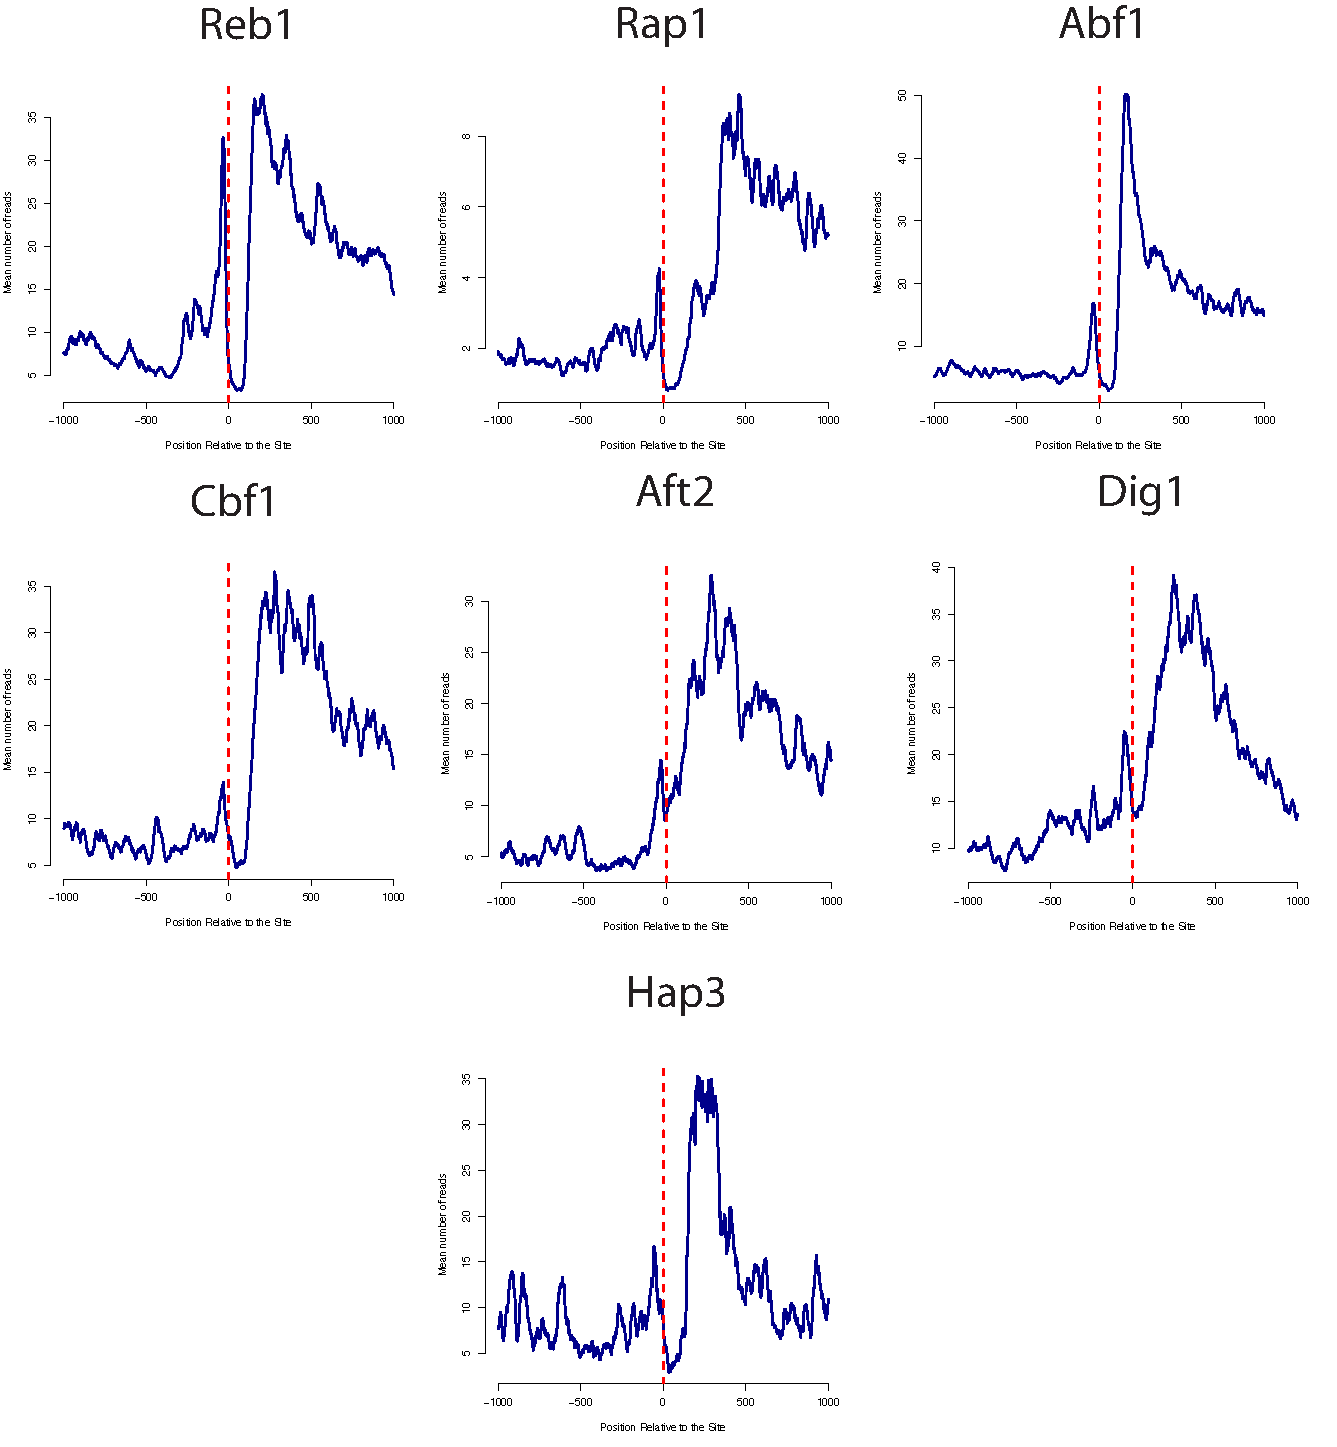
\includegraphics[width=\textwidth]{figures/results/rap/nine.pdf}
\caption[Metagene analysis around several putative road-blocking factors]{Metagene analyses performed around several putative road-blocking factors.}
\label{fig:nine}

\end{figure}
Indeed, the appearance of a peak at a given position is more stringently linked to changes that affect the whole distribution of values and less dependent on the contribution of extreme values. Consistently, a prominent and specific peak of polymerase pausing was observed by this method immediately upstream of many transcription factors (Fig. \ref{fig:nine}).  
Roadblock occurs at a variable distance between 20 and 40 nucleotides upstream of the protein binding site, likely reflecting the topology of the collision between polymerase and the DNA-bound factor or complex of factors. 

We also sought evidence of road-block termination at other sites where RNAPII transcription might collide with DNA-associated events. Prominent levels of road-block termination were observed at centromeres and tRNAs. In \cer{}, centromeres are defined by a set of short, conserved sequence elements located in a 125nt region. These sequences, CDEI, CDEII and CDEIII (Fig. \ref{fig:ten}) are specifically bound by DNA binding complexes that overall constitute the kinetochore, required for the attachment of the chromosomes to microtubules during cell division \cite[for review see][]{mckinley:2015:molecular}. The analysis of the RNAPII metaprofile around centromeres clearly indicates a prominent level of road-block when centromeres are aligned using the external CDEI or the CDEIII sequence motifs, bound respectively by Cbf1 and the Cbf3 complex. 

\begin{figure}[h]

\centering
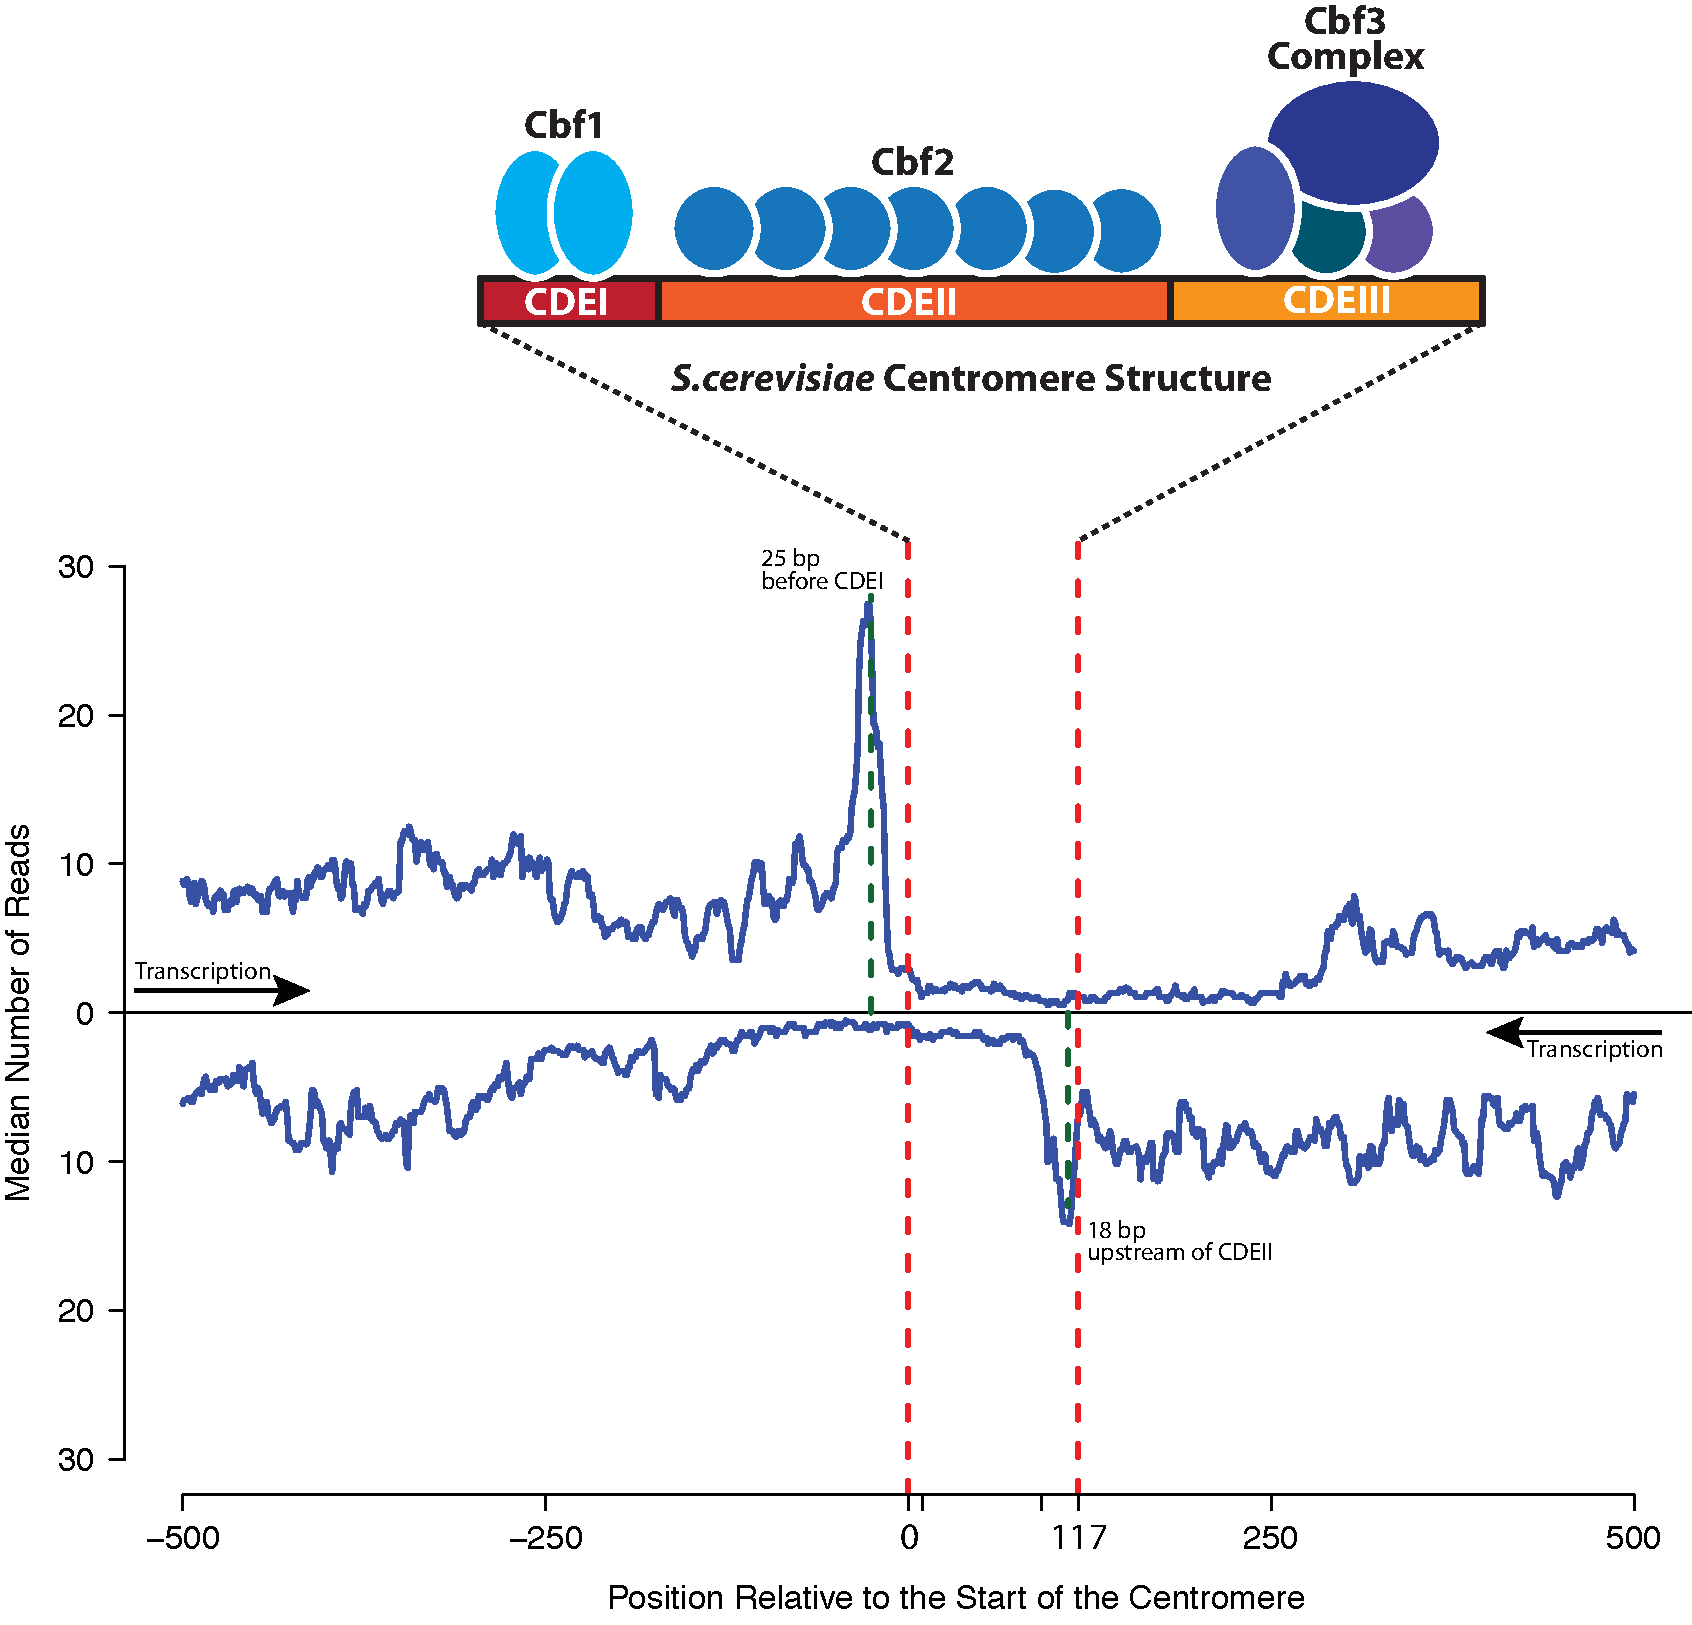
\includegraphics[width=\textwidth]{figures/results/rap/ten.pdf}
\caption[Centromere structure and polymerase occupancy profile]{Schematic representation of the structure of the centromere and the RNAPII occupancy profile around it. The top and bottom of the graph represent the two strands, the direction of transcription is indicated by arrows.}
\label{fig:ten}

\end{figure}


Prominent levels of road-block termination also occur at tRNAs. This was previously observed in the 5’-end of a model tRNA, where road-block was attributed to the binding of the RNAPIII factor TFIIIB \cite{korde:2014:intergenic}. We extended this finding genomewide, by showing RNAPIIs piling up at position -75 from the tRNA start site, corresponding to a road-block induced by TFIIIB bound at position -50 from the start site. Importantly, however, we also observed a prominent road-block antisense to the tRNA. RNAPII strongly accumulates about 50 nucleotides upstream of the annotated end of the tRNA (Fig. \ref{fig:eleven}). Because RNAPIII transcription is not known to depend on factors bound to the DNA, we infer that roadblocking occurs from the collision of RNAPII with RNAPIII, presumably paused at the termination signal or persistently occupying the tRNA transcription region. 

\begin{figure}[h]

\centering
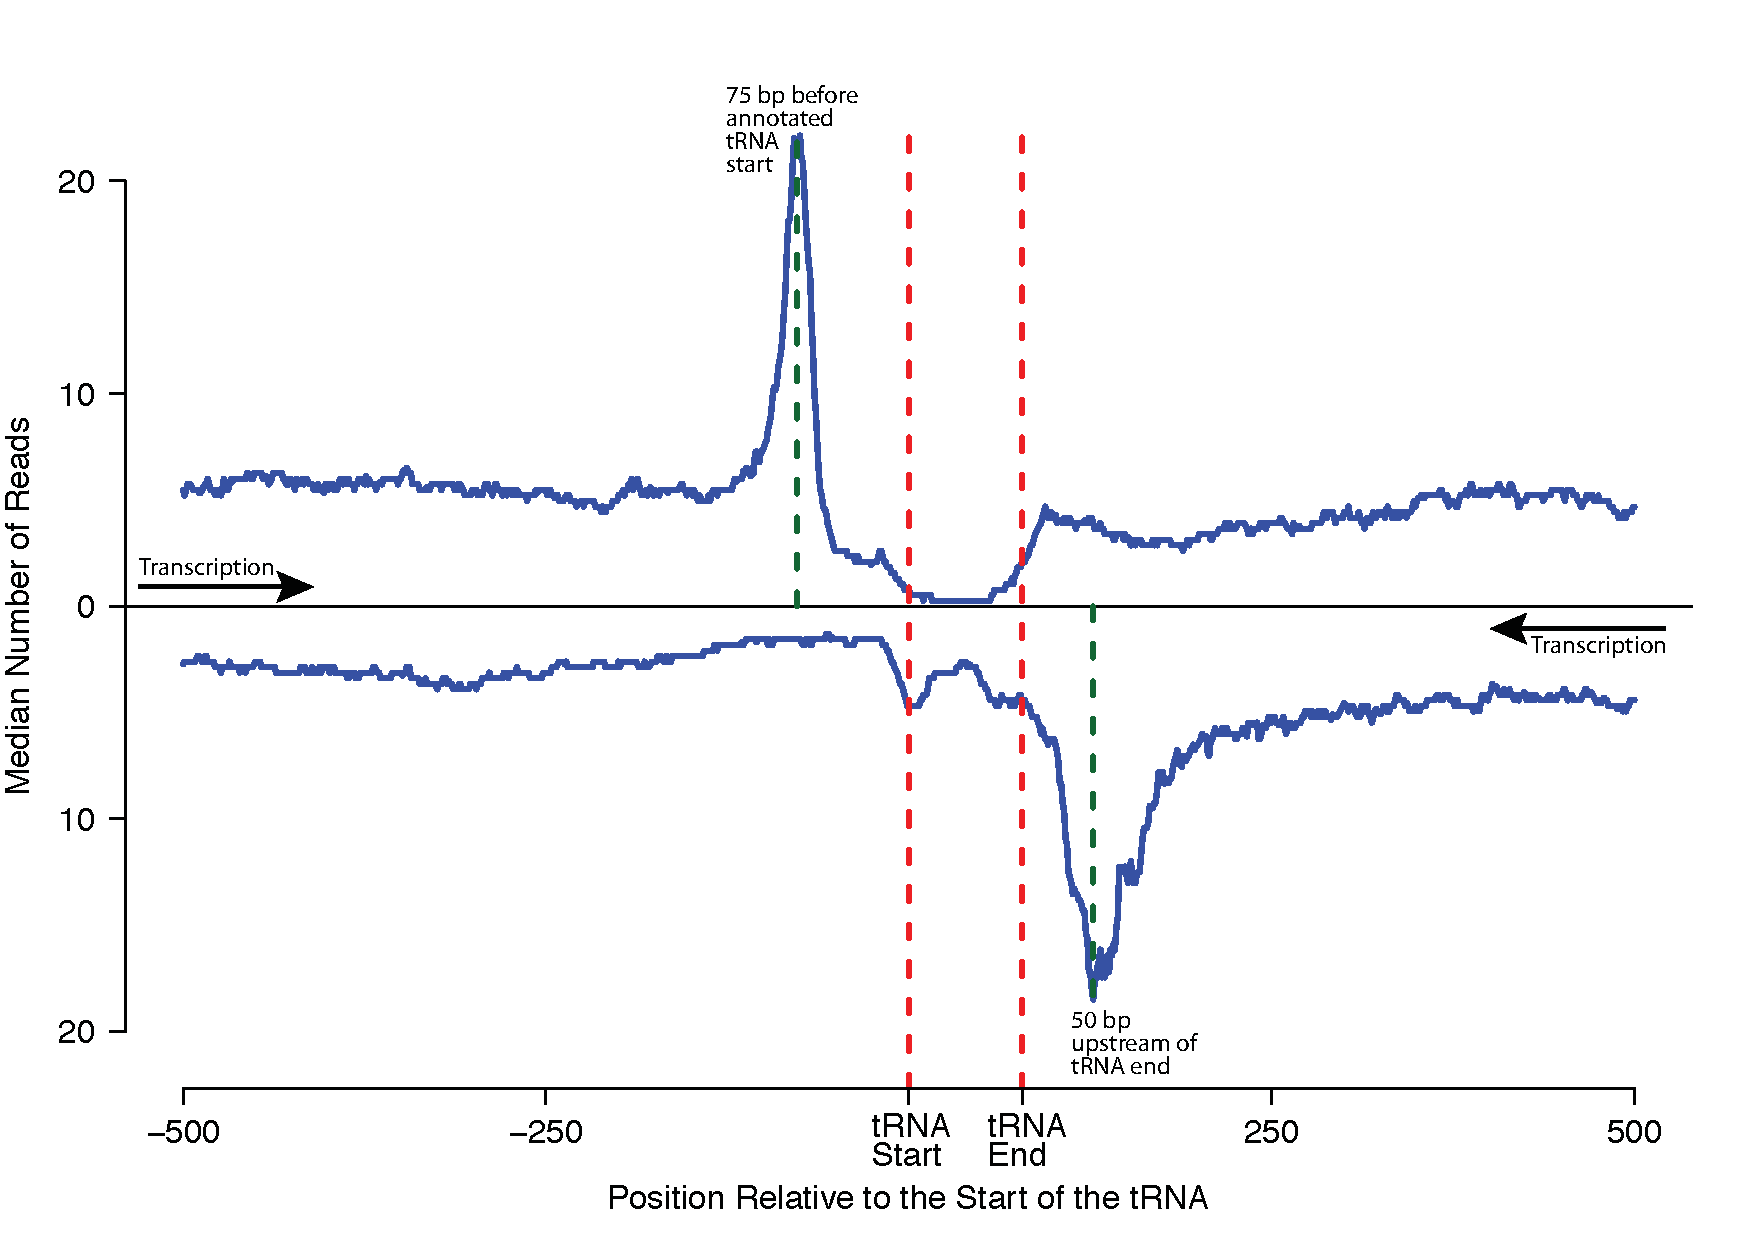
\includegraphics[width=\textwidth]{figures/results/rap/eleven.pdf}
\caption[metagene analysis of RNAPII occupancy around tRNAs]{metagene analysis of RNAPII occupancy around tRNAs. The top and bottom of the graph represent the two strands, the direction of transcription is indicated by arrows.}
\label{fig:eleven}

\end{figure}

Together, these data demonstrate that road-block termination is not restricted to Reb1 or Rap1 binding sites, but also occurs at many different locations in the yeast genome. Aside from operating a quality control mechanism on the efficiency of termination at canonical sites, road-block pausing of polymerases has potential for gene regulation and coordination of transcription with other DNA related events




\subsection{Discussion}


In a previous study we have described an additional pathway whereby transcription termination occurs when the elongation complex encounters the factor Reb1 bound to the DNA. Based on a few model cases we have proposed that road-block termination by Reb1 limits pervasive transcription and functions to “protect” promoters regions from “invading” polymerases. The general validity of these concepts was, however, not addressed in this early study. Here we extend these concepts to a genomewide perspective and to other factors, providing a general view of the impact and functional significance of road-block termination in the \cer{} genome.  

We first demonstrated that Rap1, a DNA binding factors that has roles in transcription activation, gene silencing and telomere homeostasy, is also a road-block factor. An earlier study showed that the fortuitous introduction of a Rap1 site in a Ty1 retrotransposon led to RNAPII stalling and repression of gene expression Based on the analysis of the RNA produced, which was non-adenylated and insensitive to exosome degradation, it was concluded that termination of transcription did not occur in these conditions \cite{yarrington:2012:novel}. We show that road-block termination occurs upstream of Rap1, leading to the production of RNAs that are polyadenylated by Trf4 and degraded for a large part by the nuclear exosome. We also detected non-adenylated RNAs, which most likely represents the nascent RNA associated to the polymerase that pauses before termination. Importantly, nuclear depletion of Rap1 prevents termination, indicating that the protein – and not the presence of termination signals overlapping its binding site – is responsible for ending transcription. Failure to detect the polyadenylated fraction for technical reasons in the study by Yarrington \textit{et al.} might account for the discrepancies; alternatively, termination might not occur in the Ty1 retrotransposon model for unknown reasons.


\singlespacing
\subsection*{The Mechanism of Roadblock Termination}
\doublespacing

Similar to what previously shown for Reb1 \cite{colin:2014:roadblock}, release of the polymerase stalled upstream of the road-block occurs, at least partially, as a consequence of its ubiquitylation by Rsp5 and presumably degradation. Thus, this pathway is not restricted to Reb1-dependent termination and presumably extends to all cases of road-block, in addition to events of pausing that cannot be resolved in a more “conservative” manner as previously demonstrated for polymerases encountering a DNA damage \cite{wilson:2013:ubiquitylation}. Using high resolution RNAPII occupancy data we observed very sharp peaks of stalling at the road-block sites, which is hardly compatible with more than one polymerase roadblocked, on average, at a time. This indicates that the clearance due to the Rsp5 pathway is as efficient as the building up of the peak, at least at steady state.

It has been recently proposed that the NNS pathway is required for releasing roadblocked polymerases. This claim was essentially funded on the observation that i) Nrd1 and Nab3 binding sites are frequently present at sites of road-block and ii) that peaks of polymerase stalling increase upon depletion of Nrd1 from the nucleus, which was taken as evidence that the clearance of roadblocked polymerases is affected when NNS termination is defective. Data shown in this report and in our previous study on road-block termination are not compatible with this model. The strongest counterevidence is that the insertion of an isolated Reb1 \cite{colin:2014:roadblock} or Rap1 site (this report) in a segment of the HSP104 gene lacking NNS termination signals, is sufficient for efficient RB termination. Moreover, these or similar constructs have been shown to be largely insensitive to depletion of Nrd1 and Nab3 \cite[data not shown]{colin:2014:roadblock}. 

This notion also holds for the natural cases of road-block termination in the \cer{} genome. We show that the cumulative road-block peak significantly increases upon depletion of Nrd1 only when considering road-block sites downstream of NNS, but not CPF-CF terminators (Fig. \ref{fig:six}, supplementary figure \ref{fig:S9}). Conversely, when the RB sites are downstream of CPF-CF terminators, mutation in the CPF-CF complex (but not Nrd1 depletion) increase the levels of roadbocked polymerases (figure \ref{fig:four}B and D, supplementary figure \ref{fig:S5}).  This suggests that alterations in the NNS (or CPF-CF) complexes do not affect the clearance of roadblocked polymerases, but their further accumulation upon failure to terminate at upstream NNS- (or CPF-CF) dependent genes. 

Thus, we favor a model according to which road-block termination operates independently of the NNS and CPF-CF pathways and does not allow recycling of the polymerase for further steps of transcription but leads to its degradation, together with the RNA that is produced. Such a disruptive mechanism might look uneconomical, but the concept is analogous to the seemingly useless transcription of many non-functional RNAs that are degraded rapidly after production by processing or quality control mechanisms. The energetic balance might still be favorable if the evolutionary cost of developing highly efficient, error-proof machineries is taken into consideration. In this respect, the genomewide analyses reported here strongly suggest that road-block termination is unlikely to be devoted to the generation of functional molecules, but rather to controlling a relatively low fraction of polymerases that might significantly affect the efficiency or robustness of neighboring processes.


\singlespacing
\subsection*{Functional Significance of Roadblock Termination}
\doublespacing

We have previously proposed that in a few model cases, Reb1-dependent road-block termination functions to neutralize transcription events that failed to undergo termination at upstream genes. The question addressed here is to what extent this is general, i.e. does significant transcription readthrough occur at CPF and NNS terminators genomewide and in cells that are proficient for termination. We show here that prominent roadblocks at Reb1 and Rap1 sites can be fed by polymerases that escape upstream CPF-CF and NNS-dependent termination, demonstrating the occurrence of constitutive readthrough at canonical terminators. Because we show that many DNA binding factors can road-block, to different extents, the elongation complex, polymerases overlooking canonical termination signals run into “bumpy” roads that limit their progression in intergenic regions, where they could interfere with transcription initiation or other cellular processes. The genomewide analysis of RNAPII distribution in mutants of the CPF pathway show that in most instances, readthrough polymerases accumulate in the adjacent intergenic regions, which is fully consistent with this notion [unpublished results, or Challal et al., in preparation]. 

A large wealth of evidence exists demonstrating that pervasive transcription is generated to a large extent by the leaky control of chromatin on initiation. This is particularly important for restricting the inherent bi-directionality of promoters and directing preferential initiation towards functional genes. Mutation of many chromatin remodelers or modifiers further weakens such a repressive control on initiation \cite{marquardt:2014:chromatinbased}. Leakiness in transcription termination is functionally analogous to the limited control of chromatin on initiation, in terms of the generation of pervasive transcription. In both cases, this allows transcription elongation in regions that are not necessarily producing functional transcripts and is susceptible to affect regulation of neighboring genes or other DNA-related processes, which requires its control \textit{a posteriori} by quality control pathways. In both cases, additional exposure of genomic information by transcription might confer evolutionary advantages.  

An appropriate level of readthrough transcription might allow the option of generating new and longer genes, for instance when the extended transcripts evolve to fuse contiguous ORFs or to generate polypeptide extensions to an existing factor. The regulatory potential of transcription readthrough should also not be neglected: modulation of termination efficiency might allow coordinating expression of tandem genes. Such a modulation might more easily apply over a flexible basal system whereby the efficiency of termination is not plateaued out.


\singlespacing
\subsection*{Relationships Between Road-Block and the Main Pathways of Termination in \cer{}}
\doublespacing


We considered the possibility that pausing induced by the road-block could favor upstream termination, by slowing down the progression of the polymerase and allowing catching up by “pursuing” enzymes like Sen1 or Rat1.  We reasoned that, should the model be correct, the progressive loss of polymerases due to termination upstream of the road-block is expected to be affected when the latter is removed or strongly diminished. However, the average profile of polymerases on aligned termination regions for CPF-dependent genes upstream of Reb1 or Rap1 roadblocks did not support this notion, and rather showed that termination occurred upstream with equal efficiency in the presence or absence of the road-block. Removing the latter has therefore the sole effect of allowing further progression of polymerases that have failed to terminate at the primary site. 

We also favor the notion that fail-safe termination is the main function of this pathway for sn/snoRNAs genes. The strong expression of many of these genes might more strictly require fail-safe termination to protect downstream features, which possibly explains the frequent occurrence of RB sites downstream of sn/snoRNA genes \cite{roy:2016:common}. Analogously to what observed for CPF termination, we found that upon Nrd1 depletion the downstream RB peak increases, consistent with the notion that the RB peak is fed by polymerases that fail to terminate at the primary NNS  transcription termination site (TTS). Moreover, when the RB factor is depleted we could not detect termination failure at the primary TTS, supporting the notion that the RB is not generally required for NNS termination. We did observe a significant accumulation of extended RNAs upon depletion of the road-block. However, because the RB only prevents progression of the relatively low fraction of polymerases that have escaped primary termination, it is unlikely that transcription going through the RB site fully accounts for the relatively high levels of extended RNAs observed, for instance at SNR8 and SNR39B. Rather, we favor the notion that the longer RNAs produced are stabler than the pre-snoRNA and accumulate because they escape exosomal degradation that ensues from NNS or RB termination. Whether release of polymerases at the secondary, RB termination also generates precursors that could be trimmed down to the mature snoRNA is unclear; however, we never observed a decrease in the levels of mature RNA when the RB was depleted, arguing against a significant contribution of these transcripts to the mature forms. 

We show that many proteins that bind the DNA are able to road-block the RNA polymerase, suggesting that transcriptional activity might be modeled to a large extent by non-histone proteins bound to the DNA. Besides transcription units, other features are “protected” by the RB, including tRNA and centromeres, for which we show evidence in this report, and replication origins [Candelli et al., in preparation, see chapter \ref{repRes}]. The case of tRNAs is possibly anomalous as we observe the occurrence of RB also at the 3’ end, where the specific presence of DNA-binding factors has not been described. The specific topology of these transcription units that are possibly circularized for a more efficient transcription re-initiation, or the general high persistence of RNAPIII at these sites might account for the inability of RNAPII to traverse these regions. Besides preventing interferences with RNAPIII transcription, the strong barriers provided by tRNAs might constitute major insulating elements for the protection of transcription units or other sensitive genomic features. 

The extent and the properties of road-block termination in the \cer{} genome suggest that significant regulation of gene expression and other DNA-related processes might occur as a result of the modulation of RNAPII progression, which might also apply to larger metazoan genomes. 

\clearpage

\subsection{Supplementary Figures}




\begin{suppfigure}[h!]

\centering
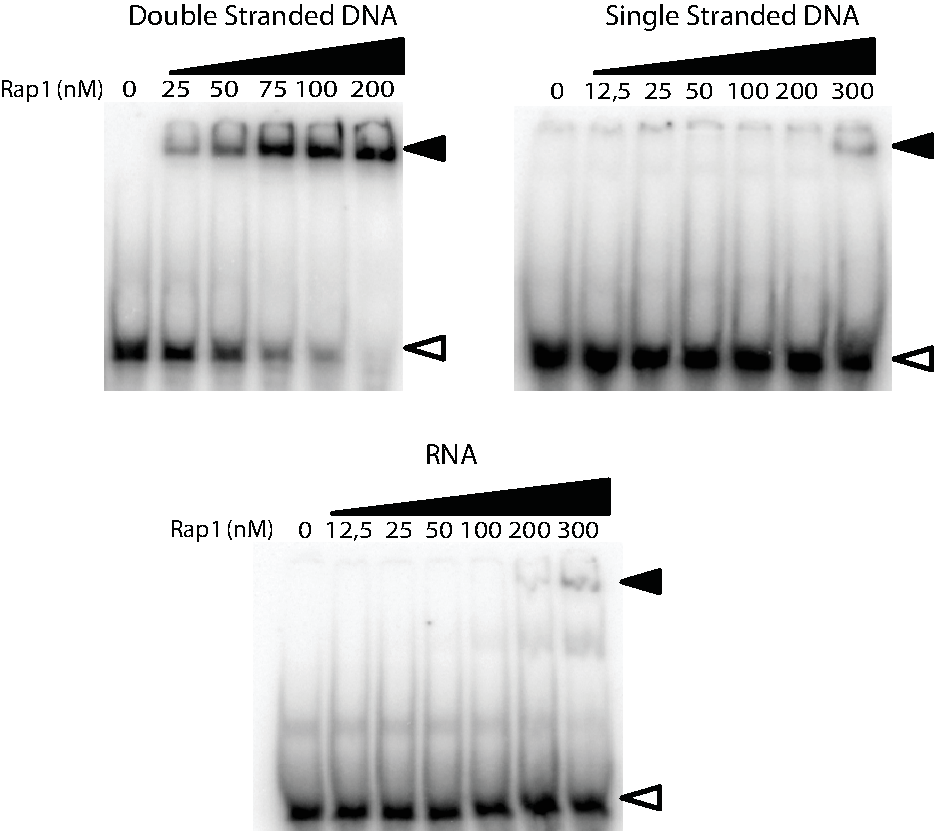
\includegraphics[width=\textwidth]{figures/results/rap/S2.pdf}
\caption[Rap1 affinity for single and double stranded DNA and RNA]{EMSA analysis of increasing concentrations of Rap1 with several species of nucleic acids: single strand DNA, double strand DNA, and RNA.}
\label{fig:S2}

\end{suppfigure}



\begin{suppfigure}[h!]

\centering
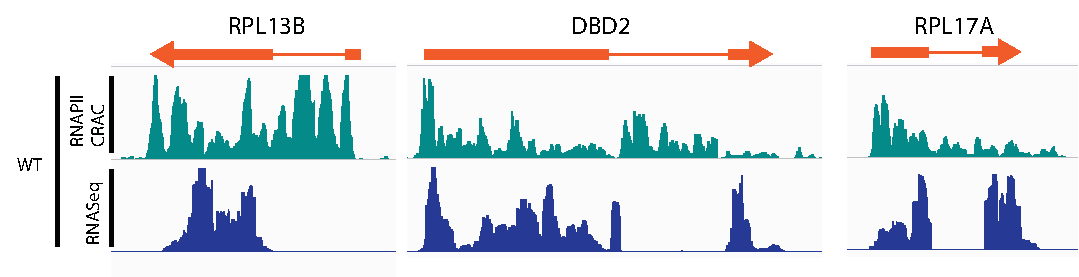
\includegraphics[width=\textwidth]{figures/results/rap/S3.pdf}
\caption[comparison between CRAC and RNA-seq signal]{Comparison between CRAC and RNA-seq signal at several loci. CRAC profiles are characterized by signal within introns.}
\label{fig:S3}

\end{suppfigure}



\begin{suppfigure}[h!]

\centering
\includegraphics[width=0.5\textwidth]{figures/results/rap/S4.pdf}
\caption[Insertion of Rap1 sites into a heterologous context]{Northern blot analysis of the insertion of two Rap1 sites within the reporter system. A short Rrp6- and Rap1-dependent transcript is present and disappears at non-permissive temperature in a Rap1 thermosensitive strain.}
\label{fig:S4}

\end{suppfigure}




\begin{suppfigure}[h!]

\centering
\includegraphics[width=\textwidth]{figures/results/rap/S5.pdf}
\caption[example of Reb1 mediated road-block]{example of Reb1-mediated road-block. CRAC signal is shown in WT-AA and Reb1-AA. RNAPII signal accumulates in proximity of Reb1 site, but this accumulation is diminished in Reb1-AA}
\label{fig:S5}

\end{suppfigure}



\begin{suppfigure}[h!]

\centering
\includegraphics[width=\textwidth]{figures/results/rap/S6.pdf}
\caption[]{metagene analysis of RNAPII PAR-CLIP signal around Reb1 sites preceded by CPF-terminated transcripts. This analysis was carried out both in a wild type and Nrd1-AA strain.}
\label{fig:S6}

\end{suppfigure}



\begin{suppfigure}[h!]

\centering
\includegraphics[width=\textwidth]{figures/results/rap/S7.pdf}
\caption[]{Metagene analysis of RNAPII CRAC around binding sites of Abf1 carried out in a wild type and rna15-1 strain at non-permissive temperature}
\label{fig:S7}

\end{suppfigure}



\begin{suppfigure}[h!]

\centering
\includegraphics[width=\textwidth]{figures/results/rap/S8.pdf}
\caption[]{Comparison between RNAPII CRAC performed in Rap1-AA + and - rapa at three Rap1 sites downstream of CPF-terminated features. Despite depletion of Rap1, no change in the efficiency of CPF termination can be detected. }
\label{fig:S8}

\end{suppfigure}



\begin{suppfigure}[h!]

\centering
\includegraphics[width=\textwidth]{figures/results/rap/S9.pdf}
\caption[dfgdf]{Metagene analyses of wild type and Nrd1-AA RNAPII PAR-CLIP signal around Rap1 and Reb1 sites preceded by NNS-terminated transcripts.}
\label{fig:S9}

\end{suppfigure}



\begin{suppfigure}[h!]

\centering
\includegraphics[width=\textwidth]{figures/results/rap/S10.pdf}
\caption[]{RT-qPCR analysis of Rap1 dependent termination upstream of the HYP2 gene. The ration between qPCR signal after and before the Rap1 sites increases significantly upon removal or Rap1.} 
\label{fig:S10}

\end{suppfigure}

\clearpage